%\documentclass[spanish,12pt,a4paper,titlepage,twoside,openright]{scrbook}
\documentclass[12pt,a4paper,titlepage]{report}
%\usepackage[latin1]{inputenc}
\usepackage[utf8]{inputenc}
\usepackage{graphicx}
\usepackage{subfig}
\usepackage{float}
\usepackage{wrapfig}
\usepackage{multirow}
\usepackage{caption}
\usepackage[spanish,es-nodecimaldot]{babel}
\usepackage[dvips]{hyperref}
\usepackage{amssymb}
\usepackage{listings}
\usepackage{epsfig}
\usepackage{amsmath}
\usepackage{array}
\usepackage[table]{xcolor}
\usepackage{multirow}
\usepackage{hhline}
\usepackage{cancel}
\usepackage{fancyvrb}

\usepackage[framed,numbered,autolinebreaks,useliterate]{mcode}

\usepackage[Sonny]{fncychap}
%\usepackage[Glenn]{fncychap}
%\usepackage[Conny]{fncychap}
%\usepackage[Rejne]{fncychap}
%\usepackage[Bjarne]{fncychap}

\usepackage{subfiles}
\usepackage{framed}
\usepackage{appendix}
\setlength{\topmargin}{-1.5cm}
\setlength{\textheight}{25cm}
\setlength{\oddsidemargin}{0.3cm} 
\setlength{\textwidth}{15cm}
\setlength{\columnsep}{0cm}
%\setkomafont{disposition}{\normalfont\bfseries}
\captionsetup{tablename=Tabla}

\ChNameVar{\bfseries\LARGE\sf}\ChNumVar{\fontsize{62}{65}\selectfont}
\ChTitleVar{\bfseries\LARGE\sf} \ChRuleWidth{2pt} \ChNameAsIs
\ChTitleAsIs
\renewcommand\FmN[4]{}
\newcommand{\HRule}{\rule{\linewidth}{0.5mm}}
\newcommand{\bs}{\boldsymbol}

\fvset{frame=single,framesep=1mm,fontfamily=courier,fontsize=\scriptsize,numbers=left,framerule=.3mm,numbersep=1mm,commandchars=\\\{\}}

\begin{document}

\begin{titlepage}
\begin{center}
\vspace{3cm}
\textsc{\LARGE Facultad de Ingenier\'ia de la Universidad de la Rep\'ublica}\\[1.5cm]
\vspace{2cm}
\textsc{\Large Introducción al Reconocimiento de Patrones  \\[1cm]  Curso 2013}\\[0.5cm]
\vspace{2cm}
% Title
\vspace{.7cm}
\HRule \\[1cm]
{ \huge \bfseries Proyecto final}\\[0.4cm]
\HRule \\[1cm]
\vspace{2cm}
% Author and supervisor

\begin{center}
\begin{tabular}{p{.5\textwidth}p{.5\textwidth}}
\emph{Autores:} & \hfill \emph{Tutores:}\\
José Luis \textsc{Nunes} &  \hfill Federico \textsc{Lecumberry}\\
Mat\'ias \textsc{Tailani\'an} & \hfill Ignacio \textsc{Ramirez}
\end{tabular}
\end{center}

\vspace{1cm}

\vfill
\begin{figure} [h!]
\centering
\subfloat{
\includegraphics[width=0.25\textwidth]{./pics/logoIIE_transparente.png}}\hspace{1cm}
\subfloat{
\includegraphics[width=0.15\textwidth]{./pics/logo_fing_transparente.png}}\hspace{1cm}
\subfloat{
\includegraphics[width=0.15\textwidth]{./pics/logo_udelar.png}}
\end{figure}

% Bottom of the page
{\large \today}
\end{center}
\end{titlepage}

\tableofcontents

\chapter{Introducción}
El objetivo principal del proyecto es la investigación en técnicas que permitan contribuir con la predicción de fertilidad de rodeo lechero y la calidad de la carne integrando técnicas de reconocimiento de patrones sobre datos de alta dimensión.\\

A lo largo de los años se ha intentado relacionar ciertas características fenotípicas del ganado bovino con algunos indicadores genéticos. Es un problema actualmente abierto de gran interés mundial y Uruguay, siendo un país esencialmente ganadero, no puede estar ajeno. Desde hace varios años se viene desarrollando una línea de investigación relacionada con la genética molecular de la calidad de la carne bovina en el área de Genética de la Facultad de Veterinaria. Se ha realizado un abordaje desde diferentes puntos de vista, como la caracterización de genes conocidos en rodeos vacunos de nuestro país, o la búsqueda y análisis de nuevos genes asociados a la calidad de carne tanto bovina como ovina \cite{bib:eileen}.\\

Obtener una correlación entre la información genética y la capacidad reprodutiva de bovinos, el impacto en la calidad de la leche y de la carne de los animales de nuestros rodeos tendría un alto impacto en la producción. A lo largo de los últimos años en Facultad de Veterinaria se han creado bases de datos con información fenotípica y genotípica relacionada conla calidad cárnica y la fertilidad bovina aplicada a la producción lechera. En esta oportunidad se trabajará con una base de datos confeccionada en nuestro país durante el año 2009, provista por la veterinaria Dra. Ana Meikle.

\chapter{Base de datos}
Para lo que sigue de este trabajo es importante conocer la base de datos con la que se trabajará, y realizar una breve descripción de las características relevantes.\\

La base de datos consta de información de un seguimiento realizado durante 9 meses sobre 891 vacas de 7 tambos diferentes y consiste en las características detalladas a continuación.

\section{Características fenotípicas}
\begin{itemize}
	\item Edad.
	\item Condición corporal (BCS) desde 30 días previos al parto hasta 120 días pos-parto, con una frecuencia de al menos una vez cada 30 días. Se utilizó la escala de 5 puntos (1=flaca, 5= gorda).
	\item Cantidad de partos (Cantidad de lactancias). Es un indicador importante que tiene que ver con la historia y desgaste de la vaca.
	\item Anestro: es la cantidad de días que pasaron desde el parto hasta el reinicio. El reinicio se define como el día en que la progesterona aumenta a un nivel determinado, indicando que la vaca volvió a ciclar.
	\item Intervalo entre partos. Es la cantidad de días que pasan entre 2 partos consecutivos (válido solamente para vacas multíparas). Para maximizar la producción de leche lo que se busca es que la vaca quede peñada una vez al año, es decir un intervalo entre partos de 365 aproximadamente.
	\item Secado: la cantidad de días que pasan entre el último día que se le saca leche a la vaca y el parto. Es válido solo para vacas multíparas. Es un indicador de cuanto tiempo se dejó descansar a la vaca antes del parto. Cuanto más tiempo tiene, se prepara el cuerpo y llega en mejor forma.
	\item Servicios: Cantidad de inceminaciones realizadas para lograr la preñez.
	\item Concentración de progesterona hasta los 60 días posparto.
	\item Promedio de cantidad de grasa en la leche durante los primeros 100 días posparto.
	\item Promedio de cantidad de leche durante los primeros 100 días posparto.
\end{itemize}

\section{Características genotípicas - Determinación de polimorfismos (SNPs)}
Se extrajo ADN y se obtuvieron muestras de buena calidad. En la figura \ref{fig:genotipo} se muestra el procedimiento realizado para caracterizar el gen IGF-I bovino en 3 clases: ``AA'', ``AB'' y ``BB''. 

\begin{figure}[H]
	\centering 
	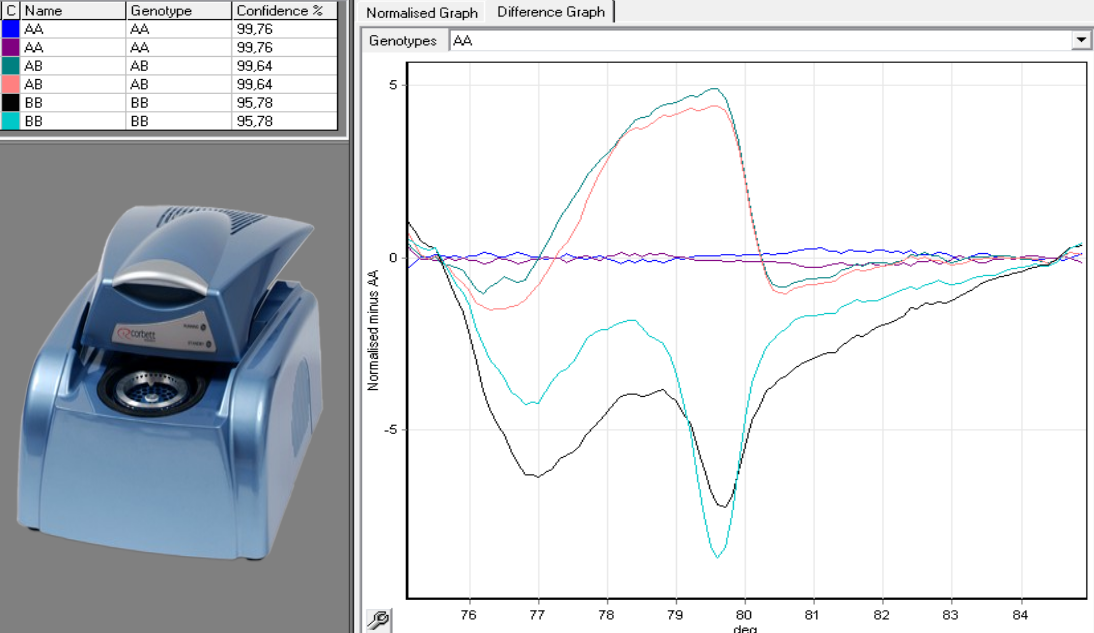
\includegraphics[width=.8\textwidth]{./pics/genotipos.png}
	\caption{Determinación del genotipo}
	\label{fig:genotipo}
\end{figure}

El eje de las ordenadas muestra la fluorescencia normalizada al genotipo ``AA''. Se puede observar que el genotipo ``AB'' se encuentra por encima del genotipo normalizado, mientras que el genotipo ``BB'' por debajo.

\section{Resumen}
En primer lugar fue necesario entender e interiorizarse con la base de datos, los conceptos y la terminología específica del problema. La lectura e interpretación de los datos no resulta para nada sencilla, por lo que se realizaron dos reuniones con la Dr. Ana Meikle, encargada de la investigación que llevó a cabo la confección de la base asociada a la producción de leche y fertilidad del ganado bovino. En ambas reuniones se buscó depurar la base con el fin de quitar información repetida y no relevante para el estudio. También se estableció un orden de relevancia en las características fenotípicas.\\

En resumen contamos con una base de datos acotada y ``limpia'' con varias características fenotípicas que se quieren correlacionar con los genotipos de cada individuo. En particular se abordará el problema como un trabajo de clasificación, tomando los genotipos como clases.

\chapter{Técnicas utilizadas}
La mayoría de los algoritmos de \emph{machine learning} seleccionan los atributos apropiados para realizar sus decisiones. Por ejemplo los métodos de árbol de desición eligen en cada paso la característica que mejor separa en clases. Cuantas más características tengamos, en teoría tendremos más poder de discriminación, pero en la práctica no ocurre así. Agregar información irrelevante o características distractivas, confunde a los algorimos de machine learning. Está probado que el número de instancias necesarias para entrenamiento para producir un cierto nivel de performance crece exponencialmente con la cantidad de atributos irrelevantes.\\

Dado el efecto negativo de las características irrelevantes es muy común en muchos algoritmos de \emph{machine learning} que se realice una etapa de selección de características donde se eliminen las irrelevantes. La mejor manera de realizar una selección de características es manual, adquiriendo un amplio conocimiento del problema en cuestión y logrando interpretar cada una de las características. Sin embargo es posible realizar una selección con algoritmos automáticos que resultan muy útiles. Reducir la dimensionalidad de los datos puede mejorar la performance de los algoritmos, además de reducir la complejidad del problema y bajar los requerimientos de capacidad de cómputo. Por esta razón se realizará una etapa de selección automática de características previa a la clasificación, como se explicará más adelante.\\ 

En una primera etapa de análisis sobre la base de datos se ataca el problema con los clasificadores \textbf{C4.5}, \textbf{Naive Bayes} y \textbf{K-NN}. \\

El algoritmo \textbf{C4.5} se utiliza para generar un árbol de desición que puede ser utilizado para clasificación. Por la naturaleza de los árboles, es un algoritmo no paramétrico, por lo que resulta robusto ante \emph{outliers}.\\

\textbf{Naive Bayes} es un clasificador basado en la aplicación del teorema de Bayes. No particiona el espacio de instancias e ignora de forma robusta a las características irrelevantes. Asume por diseño que todas las características son independientes entre si, y paga un precio muy alto cuando hay características redundantes.\\

El algoritmo \textbf{k-NN} (k-nearest neighbors) es un algoritmo de clasificación supervizado no paramétrico que pedice la clase de las instancias basado en los \emph{k} vecinos más cercanos. Es un algoritmo muy sensible a la propia estructura de los datos. Cuando $k\rightarrow \infty$, el algoritmo asegura una tasa de error no superior al doble de la tasa de error de Bayes (mínimo alcanzable dada la distribución de los datos).\\

Con esta batería de clasificadores se cubre un amplio espectro y se utilizan algunos de los algoritmos más utilizados para problemas de reconocimiento de patrones.\\

Para analizar los resultados se utilizan las implementaciones provistan en el software \textbf{Weka} \cite{bib:weka}.

\section{Primera etapa}
Se utiliza el clasificador compuesto AttributeSelectedClassifier  que aplica una técnica de selección de características antes de entrenar al clasificador. Se logra entonces una reducción de la dimensionalidad. La estrategia elegida para la selección de características se realiza utilizando el enfoque wrapper , que evalúa el set de atributos utilizando un esquema de aprendizaje y utiliza validación cruzada para estimar la precisión del esquema de aprendizaje. El clasificador utilizado para estimar esta precisión es un árbol de decisión \textbf{C 4.5}.\\

En todos los casos se utilizó validación cruzada con 10 subconjuntos.\\

Una vez hecha la extracción de características, y así la reducción de dimensionalidad, se estudia el desempeño de diferentes clasificadores. En la tabla \ref{tab:resultados_etapa1} se muestran los resultados para los algoritmos C4.5, Naive Bayes y k-NN.
\begin{table}[H]
\centering
	\begin{tabular}{c|c|c|c|c|c|} 
	\cline{2-6}
	& \multicolumn{1}{c|}{\cellcolor[gray]{0.7} \textbf{Tiempo [s]}}  
	& \multicolumn{1}{c|}{\cellcolor[gray]{0.7} $\mathbf{\sqrt{MSE}}$}
	& \multicolumn{1}{c|}{\cellcolor[gray]{0.7} \textbf{F-Measure}}
	& \multicolumn{1}{c|}{\cellcolor[gray]{0.7} $\bs\kappa$}
	& \multicolumn{1}{c|}{\cellcolor[gray]{0.7} \textbf{Bien Clasif [\%]}} \\ \hline
	
	\multicolumn{1}{|c|}{\cellcolor[gray]{0.8} \textbf{C4.5}}   & 0.84 & 0.45 & 0.331 & 0 & \cellcolor[gray]{0.9}49.83  \\ \hline
	\multicolumn{1}{|c|}{\cellcolor[gray]{0.8} \textbf{Bayes}}  & 0.37 & 0.45 & 0.345 & 0.0044 & \cellcolor[gray]{0.9}49.60 \\ \hline
	\multicolumn{1}{|c|}{\cellcolor[gray]{0.8} \textbf{k-NN}}   & 0.37 & 0.53 & 0.402 & 0.0043 & \cellcolor[gray]{0.9}45.23 \\ \hline
	\end{tabular} 
	\caption{Resultados etapa 1}
	\label{tab:resultados_etapa1}
\end{table}
Se puede observar en la tabla anterior que se obtienen resultados muy similares para los 3 algoritmos. Para C4.5 y Bayes se obtiene un porcentaje de aciertos un poco menor al 50\%, mientras que para k-NN los resultados son un poco inferiores. \\

La medida de error \emph{kappa-statistic} ($\bs\kappa$), es un indicador de la performance del algoritmo que tiene en cuenta las coincidencias por azar. Se calcula como $$\bs\kappa = \frac{P_0-P_e}{1-P_e}$$donde $P_0$ es la proporción de coincidencias observadas y $P_e$ la proporción de coincidencias esperadas en las hipótesis de independencia, es decir, coincidencias por azar. Se puede ver en la tabla \ref{tab:resultados_etapa1} que se obtuvieron valores de $\bs\kappa$ realmente bajísimos, siendo este un indicador más de la mala performance alcanzada por los algoritmos.\\

Por otro lado resulta interesante analizar las matrices de confusión que resultan de estos algoritmos. Para el C4.5 se obtiene la siguiente matriz:
\begin{lstlisting}
   a   b   c   <-- classified as								C4.5
   0 309   0 |   a = AA
   0 444   0 |   b = AB
   0 138   0 |   c = BB
\end{lstlisting}
Claramente el resultado obtenido no es el esperado. En este caso clasifica todos los patrones como pertenecientes a la clase ``AB'', y como esta clase representa casi el 50\% de todas las muestras, el porcentaje de aciertos coincide. Este es un resultado determinístico, que más allá del porcentaje de aciertos, significa que el clasificador no funcionó adecuadamente. A su vez, analizando el árbol de decisión se puede ver que tiene una sola hoja.\\

Por otro lado las matrices de confusión para los algoritmos \emph{Naive Bayes} y \emph{k-NN} son las siguientes:
\begin{lstlisting}
   a   b   c   <-- classified as							   Bayes
   6 300   3 |   a = AA
   8 435   1 |   b = AB
   1 136   1 |   c = BB
\end{lstlisting}
\begin{lstlisting}
   a   b   c   <-- classified as								k-NN
  63 233  13 |   a = AA
  81 331  32 |   b = AB
  18 111   9 |   c = BB
\end{lstlisting}
Si bien estos dos casos no se obtuvo un resultado determinístico como con C4.5, igualmente los resultados tienen un fuerte sesgo hacia la clasificación de los patrones como pertenecietes a la clase ``AB''.\\

Para mitigar el fenómeno de la salida determinística (y el sesgo) mencionado, el siguiente paso es atacar el problema del desbalance de clases. Para ello se realiza un sorteo aleatorio de las muestras pertenecientes a las 2 clases mayoritarias, de forma que las 3 clases tengan la misma cantidad de patrones. Los resultados se presentan en la siguiente sección.

\section{Segunda etapa - Clases balanceadas}

Las características seleccionadas son la condición corporal al momento del parto, a los 30, 45 y 90 días post parto, la cantidad de lactancias, la edad, el intervalo entre partos, progesterona y la cantidad de leche. \\

Los resultados de la segunda etapa, balanceando las clases, se muestran en la figura \ref{tab:resultados_etapa2}. 

\begin{table}[H]
\centering
	\begin{tabular}{c|c|c|c|c|c|} 
	\cline{2-6}
	& \multicolumn{1}{c|}{\cellcolor[gray]{0.7} \textbf{Tiempo [s]}}  
	& \multicolumn{1}{c|}{\cellcolor[gray]{0.7} $\mathbf{\sqrt{MSE}}$}
	& \multicolumn{1}{c|}{\cellcolor[gray]{0.7} \textbf{F-Measure}}
	& \multicolumn{1}{c|}{\cellcolor[gray]{0.7} $\bs\kappa$}
	& \multicolumn{1}{c|}{\cellcolor[gray]{0.7} \textbf{Bien Clasif [\%]}} \\ \hline
	
	\multicolumn{1}{|c|}{\cellcolor[gray]{0.8} \textbf{C4.5}}   & 12.57 & 0.54 & 0.39 & 0.080 & \cellcolor[gray]{0.9}38.65  \\ \hline
	\multicolumn{1}{|c|}{\cellcolor[gray]{0.8} \textbf{Bayes}}  & 11.77 & 0.50 & 0.30 & 0.044 & \cellcolor[gray]{0.9}36.23 \\ \hline
	\multicolumn{1}{|c|}{\cellcolor[gray]{0.8} \textbf{k-NN}}   & 11.92 & 0.63 & 0.38 & 0.069 & \cellcolor[gray]{0.9}37.92 \\ \hline
	\end{tabular} 
	\caption{Resultados etapa 2}
	\label{tab:resultados_etapa2}
\end{table}

Como primer ítem a mencionar se debe destacar el descenso en el porcentaje de aciertos, de algo más del 10\%. Mientas que los resultados de la primera etapa arrojaban un porcentaje de aciertos de aproximadamente 49\%, en esta etapa se nota un descenso hasta alrededor de los 38 puntos pocentuales. Aunque a priori parece un peor resultado, en interesante analizarlo con cuidado ya que por ejemplo el índice $\bs\kappa$ aumentó un órden de magnitud, aunque sigue siendo muy malo.\\

A diferencia de los resultados de la etapa anterior, para el caso del algoritmo C4.5 se obtiene un árbol no trivial con una cantidad total de 147 nodos y 74 hojas. Si bien la clasificación se encuentra por encima de una una clasificación aleatoria, son resultados realmente muy malos. \\

El balanceo de clases logró solucionar el problema del resultado determinístico (o el fuerte sesgo) donde se clasificaba todos los patrones (o casi todos) como pertenecientes a la clase ``AB'', y la matriz de confusión se muestra a continuación:
\vspace{-10pt}
\begin{lstlisting}
  a   b   c   <-- classified as									C4.5   
 44  55  39 |  a = AA
 51  54  33 |  b = AB
 40  36  62 |  c = BB
\end{lstlisting}
\vspace{-1cm}
\begin{lstlisting}
  a   b   c   <-- classified as								   Bayes
 10 102  26 |   a = AA
  6 107  25 |   b = AB
 19  86  33 |   c = BB
\end{lstlisting}
\vspace{-1cm}
\begin{lstlisting}
  a   b   c   <-- classified as									k-NN
 45  52  41 |  a = AA
 54  49  35 |  b = AB
 31  44  63 |  c = BB
\end{lstlisting}

Dado el terriblemente bajo porcentaje de aciertos obtenido en esta etapa, en la siguiente etapa se intentará realizar una extracción de características con métodos más sofisticados e intentar explicar el por qué de los resultados tan malos.

\section{Tercera etapa - extración de características}

En la tercera etapa buscaremos realizar extracción de características con el fin de reducir la dimensionalidad y  buscar características con mayor discriminación. 

Esto tiene como fin reducir los niveles de redundancia entre las características, visualizar características latentes significativas y generar para el futuro una mayor compresión en el proceso de generación de datos. 

\subsection{PCA}

El algoritmo \textbf{PCA} (Análisis de componentes principales) tiene como fin encontrar la base de vectores que mejor exprese la distribución de los datos en el espacio completo. Es similar a encontrar las componentes ortogonales de un vector en un espacio, o lo que es igual, encontrar un conjunto de vectores que combinados en forma lineal representen los elementos. Estos elementos son los vectores propios de la matriz de covarianza correspondiente al espacio original. \textbf{PCA} tiene como fin encontrar un subespacio principal en el cual se maximice la varianza de los datos proyectados. Se ordenan las variables de acuerdo a la cantidad de varianza que concentran y se utilizan solamente las más significativas.

\begin{figure} [H]
\centering
  \subfloat[Características 1-2-3]{\label{fig:pca123} 
  		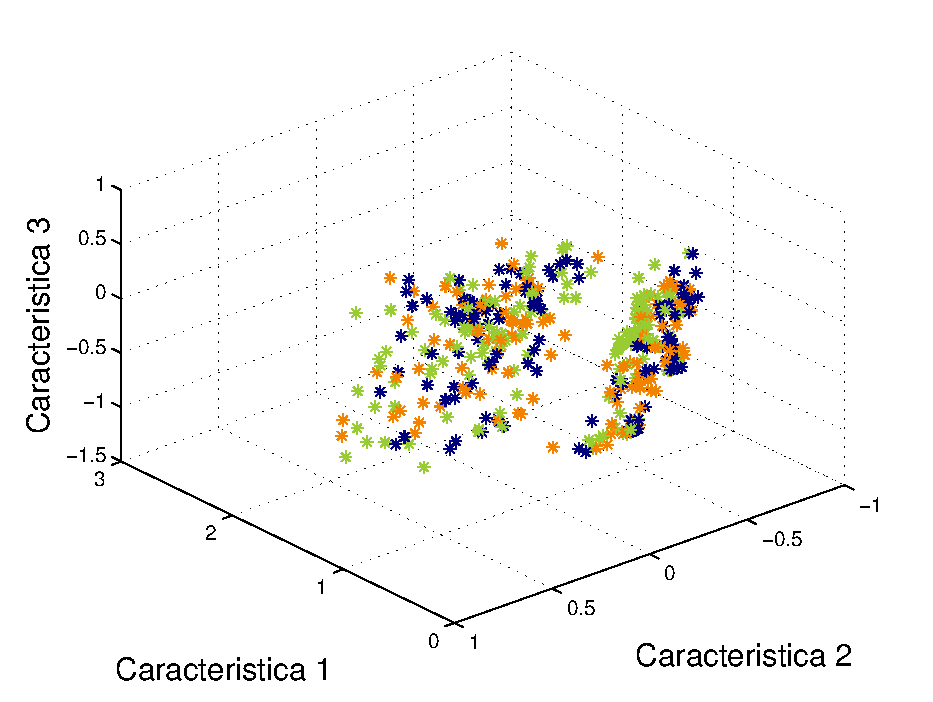
\includegraphics[width=.5\textwidth]{pics/pca123}} 
  \subfloat[Características 1-4-3]{\label{fig:pca143} 
  		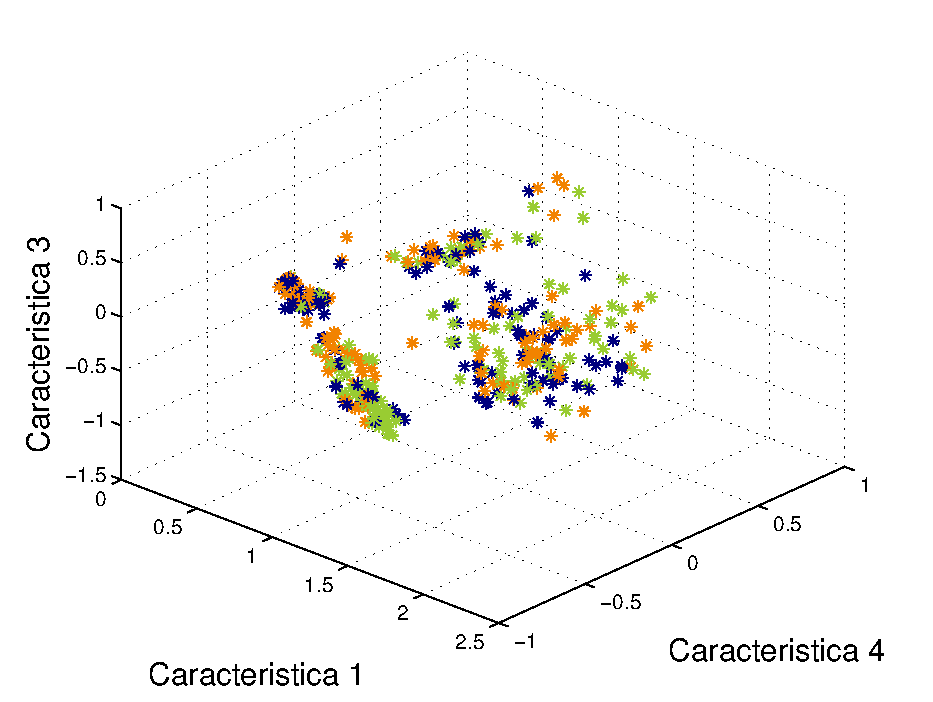
\includegraphics[width=.5\textwidth]{pics/pca143}} \\
  \caption{Datos procesados con el algorítmo PCA} 
  \label{pcas}
\end{figure}

A simple vista resulta muy difícil reconocer algún tipo de estructura sobre los datos, con lo cual es de esperar que la clasificación no entregue mejores resultados de los ya vistos. La distribución de los datos en ambos subespacios (ver figura \ref{pcas}) resulta prácticamente randómica y es imposible identificar visualmente algún cluster por clases. (Esto es medio trucho, pero sincero...)\\

\begin{wrapfigure}{l}{0.6\textwidth}
	\vspace{-25pt}
	\begin{center}
		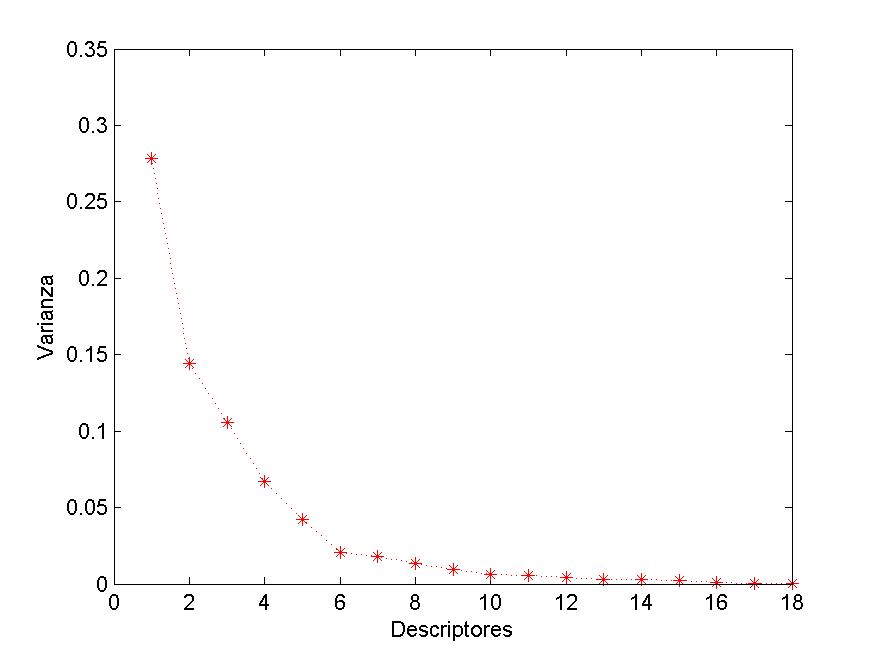
\includegraphics[width=0.5\textwidth]{pics/varianzaPCA}
	\end{center}
	\vspace{-20pt}
	\caption{Varianza vs Componentes}
	\label{varianzaPCA}
	\vspace{-10pt}
\end{wrapfigure}

En la figura \ref{varianzaPCA} vemos la varianza en función de los componentes, podemos apreciar como la caída es abrupta y tiene sentido trabajar en el espacio de los primeros tres componentes que acumulan la mayor cantidad de varianza.\\

Los resultados de aplicar los clasificadores a los datos procesados con PCA se muestran en la tabla \ref{tab:resultados_PCA}.
\begin{table}[H]
\centering
	\begin{tabular}{c|c|c|c|} 
	\cline{2-4}
	& \multicolumn{1}{c|}{\cellcolor[gray]{0.7} \textbf{Tiempo [s]}}  
	& \multicolumn{1}{c|}{\cellcolor[gray]{0.7} $\bs\kappa$}
	& \multicolumn{1}{c|}{\cellcolor[gray]{0.7} \textbf{Bien Clasif [\%]}} \\ \hline
	
	\multicolumn{1}{|c|}{\cellcolor[gray]{0.8} \textbf{C4.5}}   & 0.03 & 0.143 & \cellcolor[gray]{0.9}42.75  \\ \hline
	\multicolumn{1}{|c|}{\cellcolor[gray]{0.8} \textbf{Bayes}}  & 0.02 & 0.091 & \cellcolor[gray]{0.9}39.37 \\ \hline
	\multicolumn{1}{|c|}{\cellcolor[gray]{0.8} \textbf{k-NN}}   & 0    & 0.149 & \cellcolor[gray]{0.9}43.24 \\ \hline
	\end{tabular} 
	\caption{Resultados etapa 2}
	\label{tab:resultados_PCA}
\end{table}
Las matrices de confusión para cada clasificador son:
\vspace{-10pt}
\begin{lstlisting}
  a  b  c   <-- classified as									C4.5
 50 42 46 |  a = 1
 43 59 36 |  b = 2
 39 31 68 |  c = 3
\end{lstlisting}
\vspace{-1cm}
\begin{lstlisting}
  a  b  c   <-- classified as								   Bayes
 19 93 26 |  a = 1
 22 85 31 |  b = 2
 18 61 59 |  c = 3
\end{lstlisting}
\vspace{-1cm}
\begin{lstlisting}
  a  b  c   <-- classified as									k-NN
 58 45 35 |  a = 1
 44 59 35 |  b = 2
 44 32 62 |  c = 3
\end{lstlisting}

Como era de esperarse analizando la distribución de los datos, se obtuvieron resultados muy malos, aunque sensiblemente mejores que en la etapa anterior, llegando en el caso de \emph{k-NN} a un porcentaje de aciertos de un poco más del 43\%.\\

A su vez, la medida estadística $\bs\kappa$ aumentó un orden de magnitud respecto a la etapa anterior, y dos órdenes respecto a la etapa 1.

\subsection{LDA}
El algorítmo LDA (Análisis de discriminantes lineales) tiene como fin seleccionar una proyección que maximice separabilidad inter-clases. Busca una proyección de los datos en un espacio de menor (o igual) dimensión que las iniciales con el fin de que la disciminabilidad inter-clases sea lo más alta posible. Es una técnica supervisada ya que para poder buscar dicha proyección se debe entrenar el sistema con patrones etiquetados.\\

\begin{figure}
	\centering 
	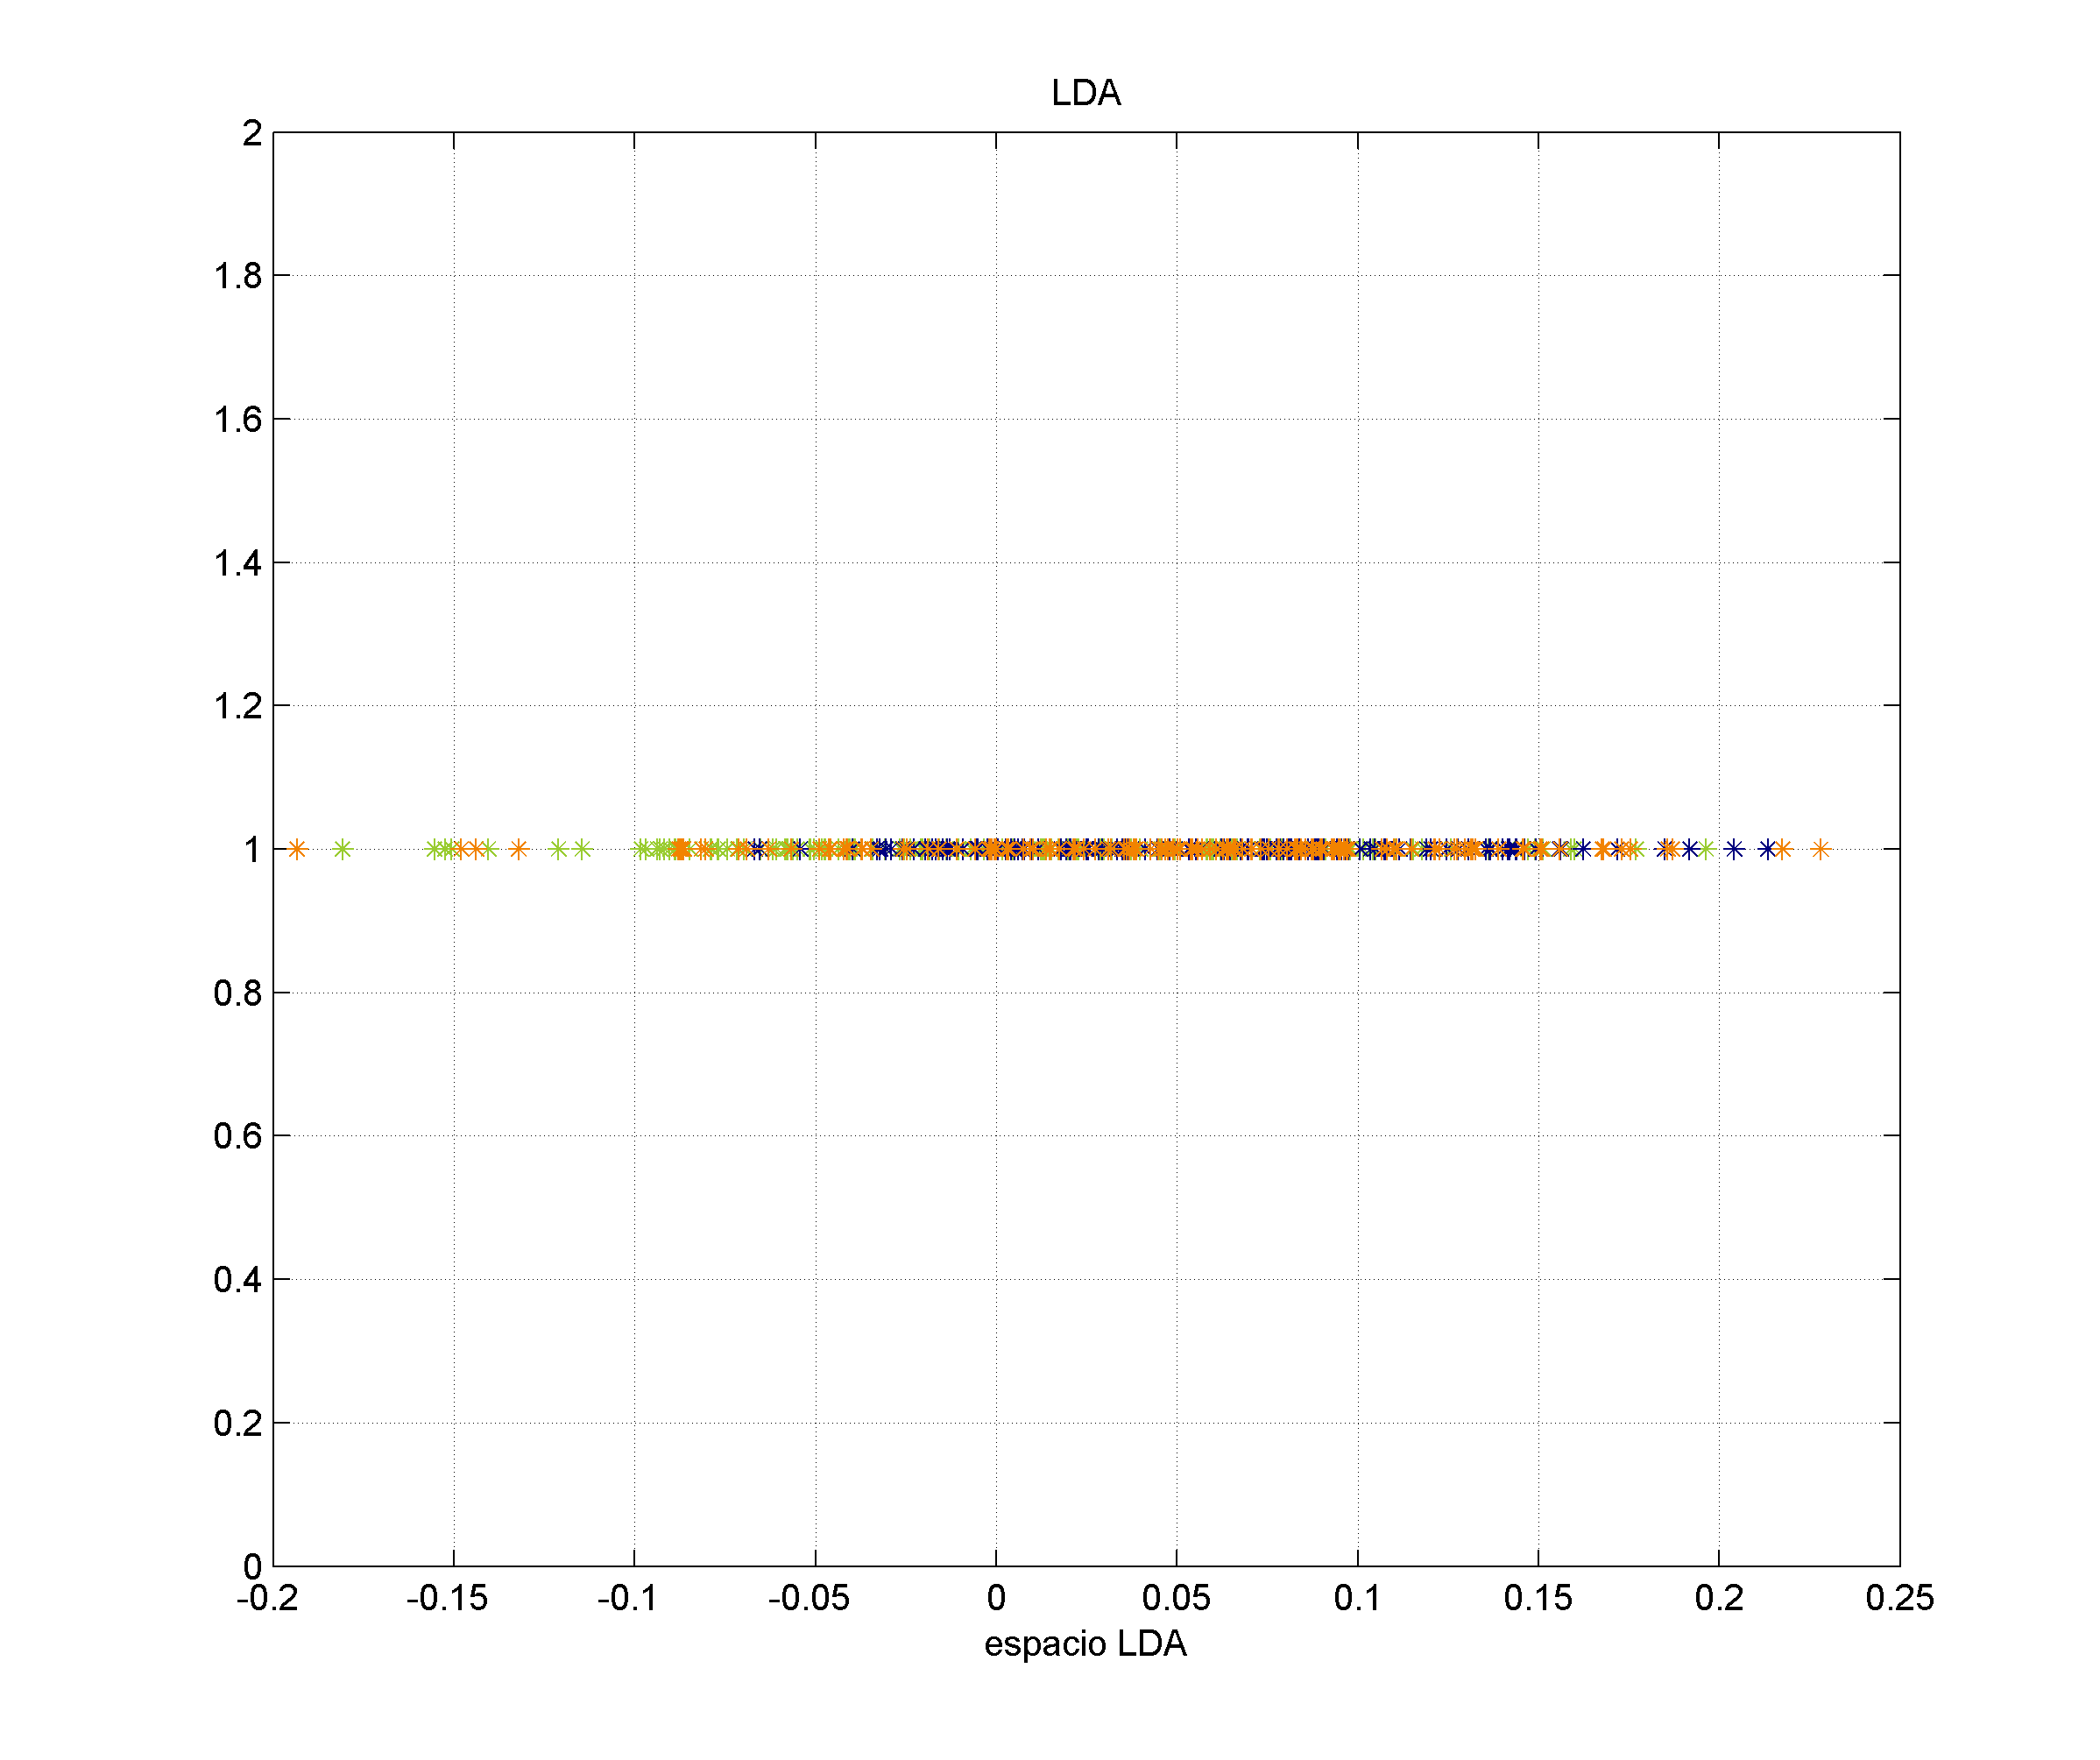
\includegraphics[width=.8\textwidth]{pics/lda2}
	\caption{Proyeccion de los datos aplicando LDA}
	\label{fig:lda}
\end{figure}

En la figura \ref{fig:lda} se muestran los resultados de aplicar LDA a los datos. Nuevamente resulta imposible obtener algun resultado visualizando la distribución de los datos, pero de todas formas se intenta realizar una clasificación con los algoritmos C4.5, Naive Bayes y k-NN. Estos resultados se muestran en la tabla \ref{tab:resultados_LDA}

\begin{table}[H]
\centering
	\begin{tabular}{c|c|c|c|} 
	\cline{2-4}
	& \multicolumn{1}{c|}{\cellcolor[gray]{0.7} \textbf{Tiempo [s]}}  
	& \multicolumn{1}{c|}{\cellcolor[gray]{0.7} $\bs\kappa$}
	& \multicolumn{1}{c|}{\cellcolor[gray]{0.7} \textbf{Bien Clasif [\%]}} \\ \hline
	
	\multicolumn{1}{|c|}{\cellcolor[gray]{0.8} \textbf{C4.5}}   & 0.03 & 0.1558 & \cellcolor[gray]{0.9} 43.7198  \\ \hline
	\multicolumn{1}{|c|}{\cellcolor[gray]{0.8} \textbf{Bayes}}  & 0 & 0.1667 & \cellcolor[gray]{0.9} 44.4444 \\ \hline
	\multicolumn{1}{|c|}{\cellcolor[gray]{0.8} \textbf{k-NN}}   & 0 & 0.1196 & \cellcolor[gray]{0.9} 41.3043 \\ \hline
	\end{tabular} 
	\caption{Resultados etapa 2}
	\label{tab:resultados_LDA}
\end{table}

Como era de esperarse al analizar los patrones en el espacio transformado, nuevamente no es posible realizar una buena clasificación con ninguno de los clasificadores probados.

Las matrices de confusión para cada clasificador son:
\vspace{-10pt}
\begin{lstlisting}
  a  b  c   <-- classified as									C4.5
  7 107 24 |  a = 1
 12 122  4 |  b = 2
  5  81 52 |  c = 3
\end{lstlisting}
\vspace{-1cm}
\begin{lstlisting}
  a  b  c   <-- classified as								   Bayes
 10 85 43 |  a = 1
  7 94 37 |  b = 2
  3 55 80 |  c = 3
\end{lstlisting}
\vspace{-1cm}
\begin{lstlisting}
  a  b  c   <-- classified as									k-NN
 64 48 26 |  a = 1
 66 54 18 |  b = 2
 43 42 53 |  c = 3
\end{lstlisting}

%TODO estimación de densidades

\subsection{Diffusion Maps}
Con el objetivo de probar alguna técnica más sofisticada se utiliza Diffusion Map \cite{bib:diffmaps}.\\

Diffusion maps es un algoritmo de \emph{machine learning} que computa una familia de conjuntos de datos en un espacio embebido, usualmente de baja dimensión, cuyas coordenadas pueden ser calculadas de los vectores y valores propios de un operador de difusión de los datos. La distancia euclídea entre puntos en el espacio embebido es la ``distancia de difusión''. A diferencia de otros métodos de reducción de dimensionalidad como PCA, este algoritmo es un método no lineal que se centra en descubrir \emph{manifold} subyacente al muestreo de los datos. Integrando la similitud local de los datos a diferentes escalas, \emph{diffusion maps} da una descripción global de los datos. Es robusto ante perturbaciones ruidosas y computacionalmente barato.\\

Los resultados de pasar a un espacio de 3 dimensiones (para poder visualizarlo) se muestran en la figura \ref{fig:dm}.
\begin{figure}[H]
	\centering 
	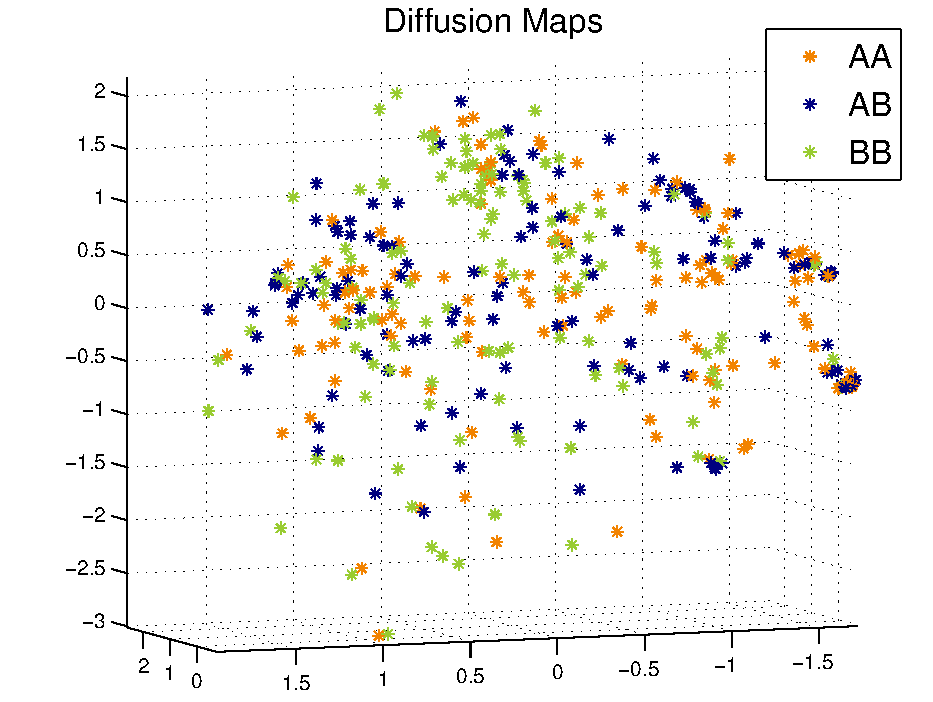
\includegraphics[width=.8\textwidth]{./pics/dm.pdf}
	\caption{Diffusion Maps}
	\label{fig:dm}
\end{figure}

Como se puede apreciar en la figura, al igual que en los casos anteriores los patrones de las diferentes clases están realmente muy entreverados, no pudiéndose diferenciar ningún cluster.


\chapter{Conclusiones}
falta\\
- hacer andar el lda y hacer la grafiquita\\
- student y anova\\
- llenar la tabla de lda\\
- conclusiones
- agregar referencia a diffusion maps

decir que vamos a seguir intentando porque excede este trabajo. mencionar wombat.



\begin{thebibliography}{99}
\begin{small}

\bibitem{bib:eileen}Eileen Armstrong Reborati, \emph{Detección y análisis de genes asociados a la calidad de la carne en bovinos}, Tesis de doctorado, Madrid, 2011.
\bibitem{bib:weka}Mark Hall, Eibe Frank, Geoffrey Holmes, Bernhard Pfahringer, Peter Reutemann, Ian H. Witten (2009); The WEKA Data Mining Software: An Update; SIGKDD Explorations, Volume 11.
\bibitem{bib:REML}Meyer, K. (2007). WOMBAT – A tool for mixed model analyses in quantitative genetics by REML, J. Zhejiang Uni.
\bibitem{bib:diffmap}R.R.Coifman, S.Lafon, A.B.Lee, M.Maggioni, B.Nadler, F.Warner y S.W.Zucker (2005). Geometric diffusions as a tool for harmonic analysis and structure definition of data: Diffusion maps.

\end{small}
\end{thebibliography}





\end{document}

\begin{wrapfigure}{l}{0.6\textwidth}
	\vspace{-20pt}
	\begin{center}
		\includegraphics[width=0.45\textwidth]{./pics/.pdf}
	\end{center}
	\vspace{-20pt}
	\caption{}
	\label{}
	\vspace{-10pt}
\end{wrapfigure}


\begin{figure} [H]
\centering
  \subfloat[Características 1]{\label{fig:c1} 
  		\includegraphics[width=.5\textwidth]{./pics/carac1.pdf}} 
  \subfloat[Características 2]{\label{fig:c2} 
  		\includegraphics[width=.5\textwidth]{./pics/carac2.pdf}} \\
  \caption{Histogramas de las características} 
  \label{fig:c1yc2}
\end{figure}


\begin{figure}[H]
	\centering 
	\includegraphics[width=.8\textwidth]{./pics/ej2_voronoi_12_coloreada.pdf}
	\caption{Voronoi - Características 1 y 2}
	\label{fig:voronoi12}
\end{figure}
